\documentclass[SE,lsstdraft,authoryear,toc]{lsstdoc}
\input{meta}

% Package imports go here.

% Local commands go here.

%If you want glossaries
%\input{aglossary.tex}
%\makeglossaries
\usepackage{amsmath}

\title{M1M3 temperature analysis under mirror transportation}

% This can write metadata into the PDF.
% Update keywords and author information as necessary.
\hypersetup{
    pdftitle={M1M3 temperature analysis under mirror transportation},
    pdfauthor={Karla Peña Ramírez},
    pdfkeywords={}
}

% Optional subtitle
% \setDocSubtitle{A subtitle}

\author{%
Karla Peña Ramírez
}

\setDocRef{SITCOMTN-141}
\setDocUpstreamLocation{\url{https://github.com/lsst-sitcom/sitcomtn-141}}

\date{\vcsDate}

% Optional: name of the document's curator
% \setDocCurator{The Curator of this Document}

\setDocAbstract{%
M1M3 monitoring temperature changes while its transportation and once it is inside the dome, is key to ensure that the mirror is within its safety limits. In this Technote I analyze temperature values from a series of sensors located in the different locations including level 3, the M1M3 cell, the hydraulic vertical lift structure, the dome at level 8 and the weather station. 
}

% Change history defined here.
% Order: oldest first.
% Fields: VERSION, DATE, DESCRIPTION, OWNER NAME.
% See LPM-51 for version number policy.
\setDocChangeRecord{%
  \addtohist{1}{YYYY-MM-DD}{Unreleased.}{Karla Peña Ramírez}
}


\begin{document}

% Create the title page.
%\maketitle
\mkshorttitle %to remove the extra pages

% ADD CONTENT HERE
% You can also use the \input command to include several content files.

\section{Introduction}
Keeping thermally safe M1M3 is paramount to ensure the optical performance required by the project. The known thermal stress requirements for M1M3 are:
\begin{enumerate}
  \item Less than 5\,\textdegree C in temperature variation in the glass surface.
  \item Temperature in the mirror can not change more than 1\,\textdegree C per hour.
\end{enumerate}

For mirror transportation, the above mentioned requirements are fulfilled if the temperature differences between two locations are $\leq\,$5 \textdegree C and by avoiding leaving the mirror in locations where temperature changes more than 1\,\textdegree C \backslash hr.

The locations involved in mirror transportation include level 3 (L3) where M1M3 was located until the date of transportation, the hydraulic vertical lift structure (p-flow), the exterior (top of the lift with the mirror raised) and level 8 (L8), where the mirror will be parked on the Telescope Mount Assembly (TMA).

With the goal of evaluating the safety limits on M1M3 transport to the dome and its temperature once it is installed at the Simonyi Telescope we are interested in retrieving temperature information from two main sets of sensors:

\begin{enumerate}
  \item \textbf{Sensor Set 1}: Environmental.
  \begin{itemize}
    \item ESS:103 (MTDome).
    \begin{description}
      \item This sensor is located inside the dome and in the proximity of M1M3.
      \item[Note:] From October 9 2024 it is renamed as ESS:113. It is the M1M3 humidity sensor.
      \end{description}
    \item ESS:301 (Weather station tower).
  \end{itemize}
  \item \textbf{Sensor Set 2}: Local temperature loggers.
  \begin{itemize}
    \item M1M3 interior cass (center).
    \item M1M3 interior $+x$.
    \item M1M3 interior $-x$.
    \item M1M3 exterior cell.
    \item M1M3 ambient at L3.
    \item Lift ambient (p-flow rail).
  \end{itemize}
\end{enumerate}

In addition to the above mentioned sensors there were two temporal local temperature loggers that were dedicated to monitor the air temperature gradient and the surrogate surface temperature gradient between L3 and L8. The temporal local temperature loggers were UPS battery powered and the probes were lifted up and down between L3 and L8. Given the short time span of the test, the conclusions derived from these loggers were incloclusive and are not included in this document.

\section{Related Test Cases}
\label{sec_test_cases}

Complementary, three Test Cases were designed and executed with the goal of study the temperature equalization between L3 and L8.

\begin{enumerate}
  \item \href{https://rubinobs.atlassian.net/projects/BLOCK?selectedItem=com.atlassian.plugins.atlassian-connect-plugin:com.kanoah.test-manager__main-project-page#!/v2/testCase/BLOCK-T172}{Test Case T172}: Dome Cooling with Air Handlers Units (AHU/UMA) 1 and 2.
  \begin{description}
    \item[Note:] Executed between September 26 and September 27. It included daytime activities.
  \end{description}
  \item \href{https://rubinobs.atlassian.net/projects/BLOCK?selectedItem=com.atlassian.plugins.atlassian-connect-plugin:com.kanoah.test-manager__main-project-page#!/v2/testCase/BLOCK-T176}{Test Case T176}: MTDome thermal flushing.
  \begin{description}
    \item[Note:] Executed on October 1 during nightime activities. It consisted on opening the dome shutters and activating the downdraft system on L5.
  \end{description}
  \item \href{https://rubinobs.atlassian.net/projects/BLOCK?selectedItem=com.atlassian.plugins.atlassian-connect-plugin:com.kanoah.test-manager__main-project-page#!/v2/testCase/BLOCK-T177}{Test Case T177}: L3 thermal flushing.
  \begin{description}
    \item[Note:] Executed on September 30 during nightime activities. It consisted on the opening/closing the p-flow roll up doors on L3.
  \end{description}
\end{enumerate}

\section{Related Tickets}
The ticket that triggered this Technote originally was designed to trace back temperature data on Sep/Oct in previous years possibility expecting to see a seasonal trend.  Nevertheless, it was rescoped towards the analysis of the current year trend.

\href{https://rubinobs.atlassian.net/browse/SITCOM-1600}{OBS-1600}: \textit{Historical analysis of the temperature on Level 8 (ESS:103) and on the Weather Station (ESS:301) in Sep/Oct last years.}


\section{Results}
\subsection{Sensor Set 1: Environmental.}
The sensors were studied from August 14 to October 2. The mirror transportation started on October 2 at 12:15 local time. Prior the movement, sensor ESS:103 monitored the temperature inside the dome close to the future location of M1M3. Figure \ref{fig_set1_difference} shows the difference in temperature between sensor ESS:103 and the weather station resampling each hour. In the left figure it can be seen that the thermal requirement of less than 5\,\textdegree C in temperature variation in the glass surface was surprased multiple times. Nevertheless, the sensor monitors the air temperature around the cell (future) location and not the glass surface. Beside this, the thermal excess (temperature $\leq$\,$\pm$5\,\textdegree C) was linked to the aperture of the rear access door (RAD) and p-flow. Possibly also linked to dome shutter apperture, still manual with no telemetry, at the moment of writting. This behaviour triggered the Test Cases mentioned on Section \ref{sec_test_cases}. It is worth to note (see Figure \ref{fig_set1_difference}, right) that the mirror movement started when the temperature difference studied here was null.

\begin{figure}[h!]
  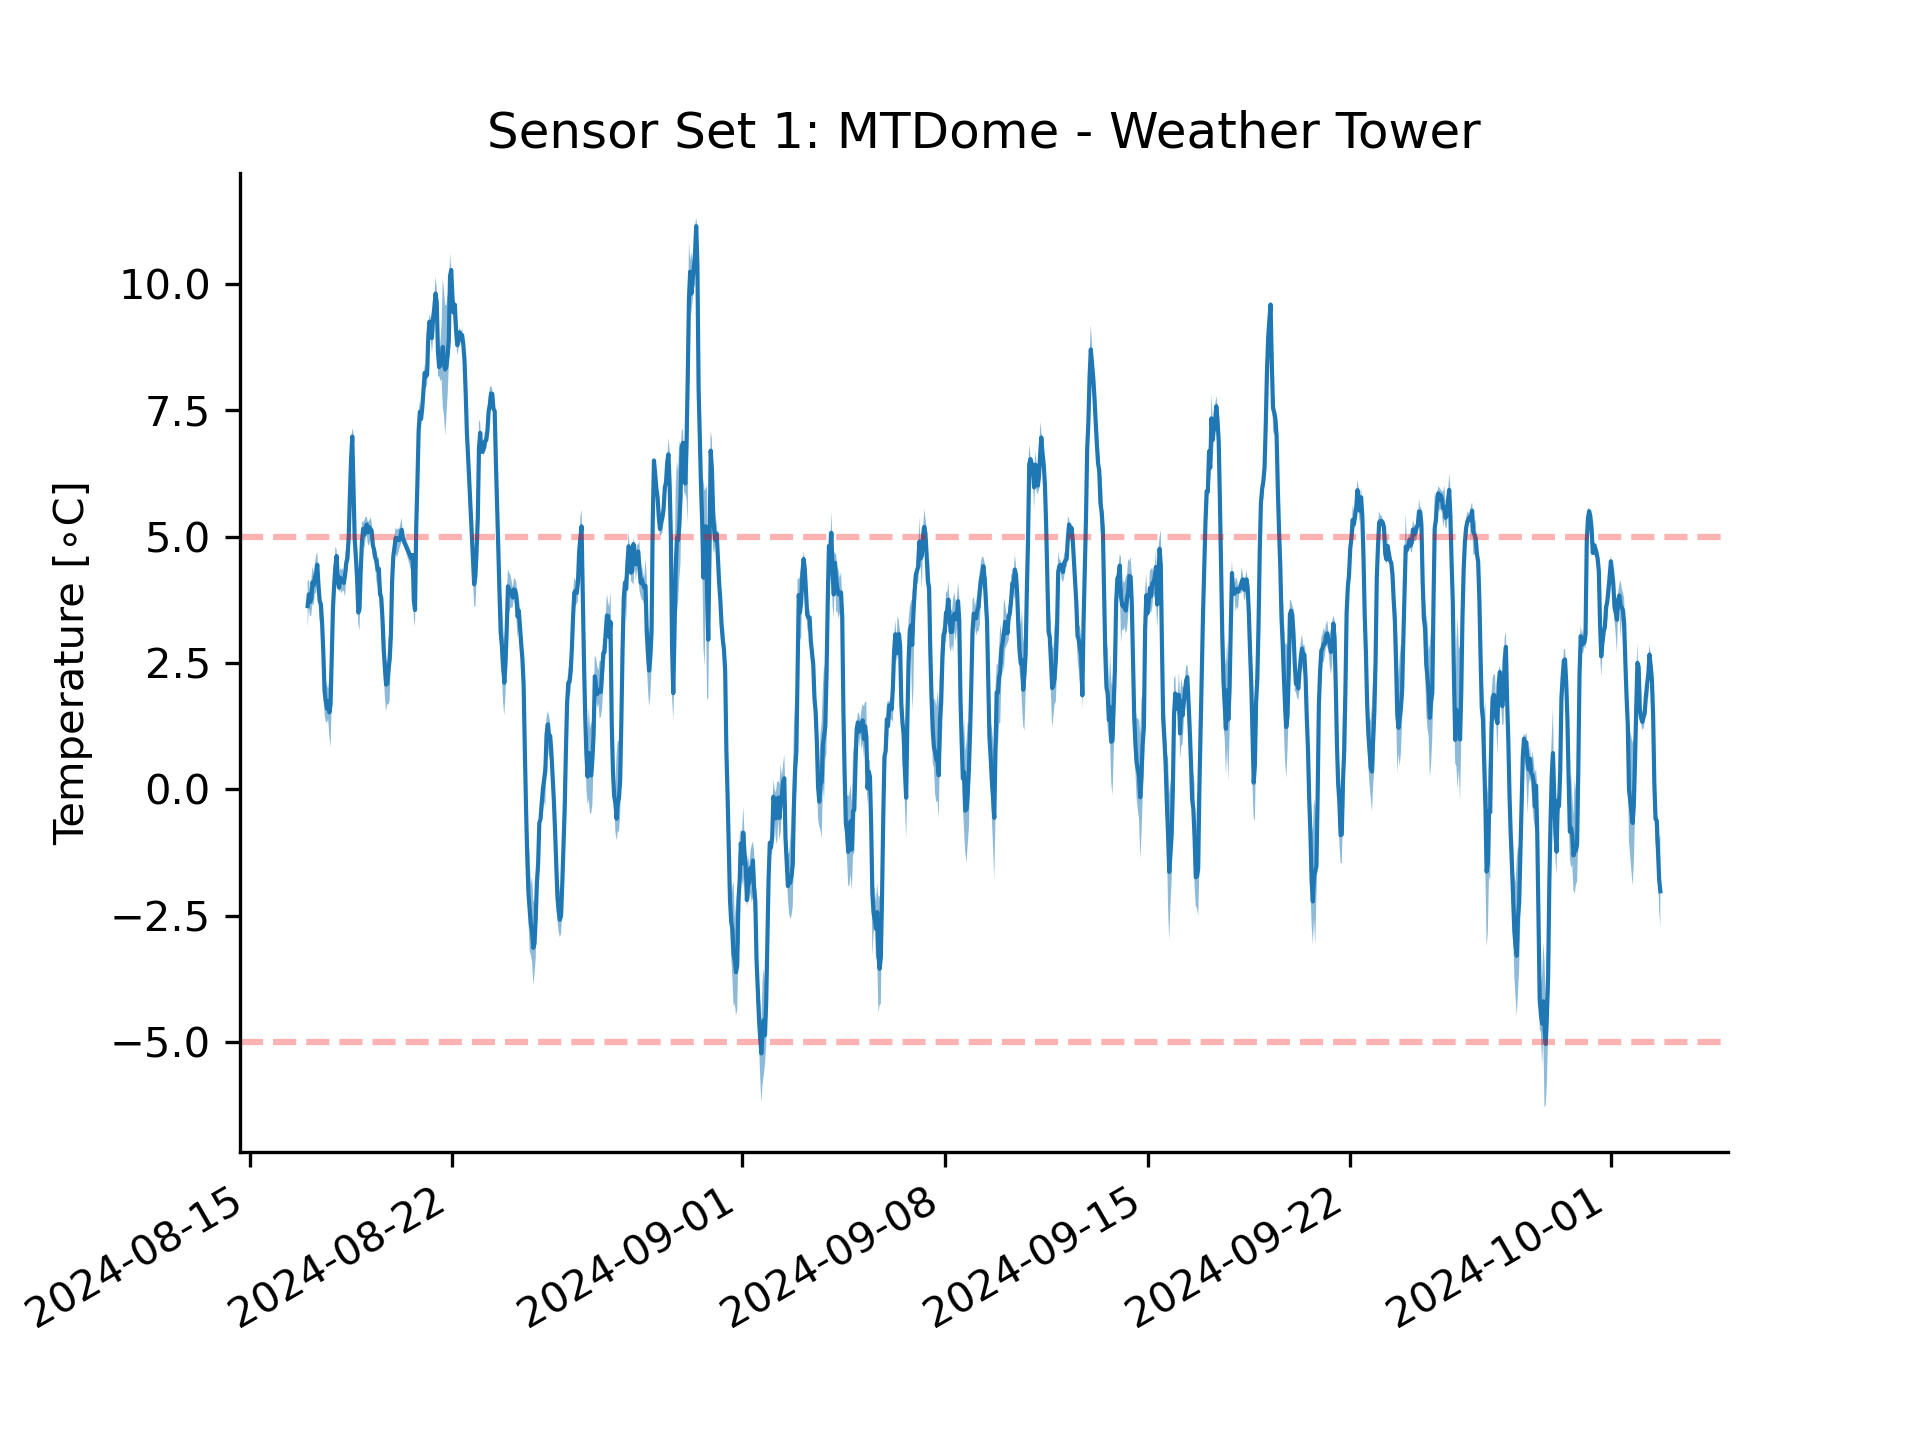
\includegraphics[width=8cm]{SITCOMTN-141_figures/Sensor1_1h_delta_temp.png}
  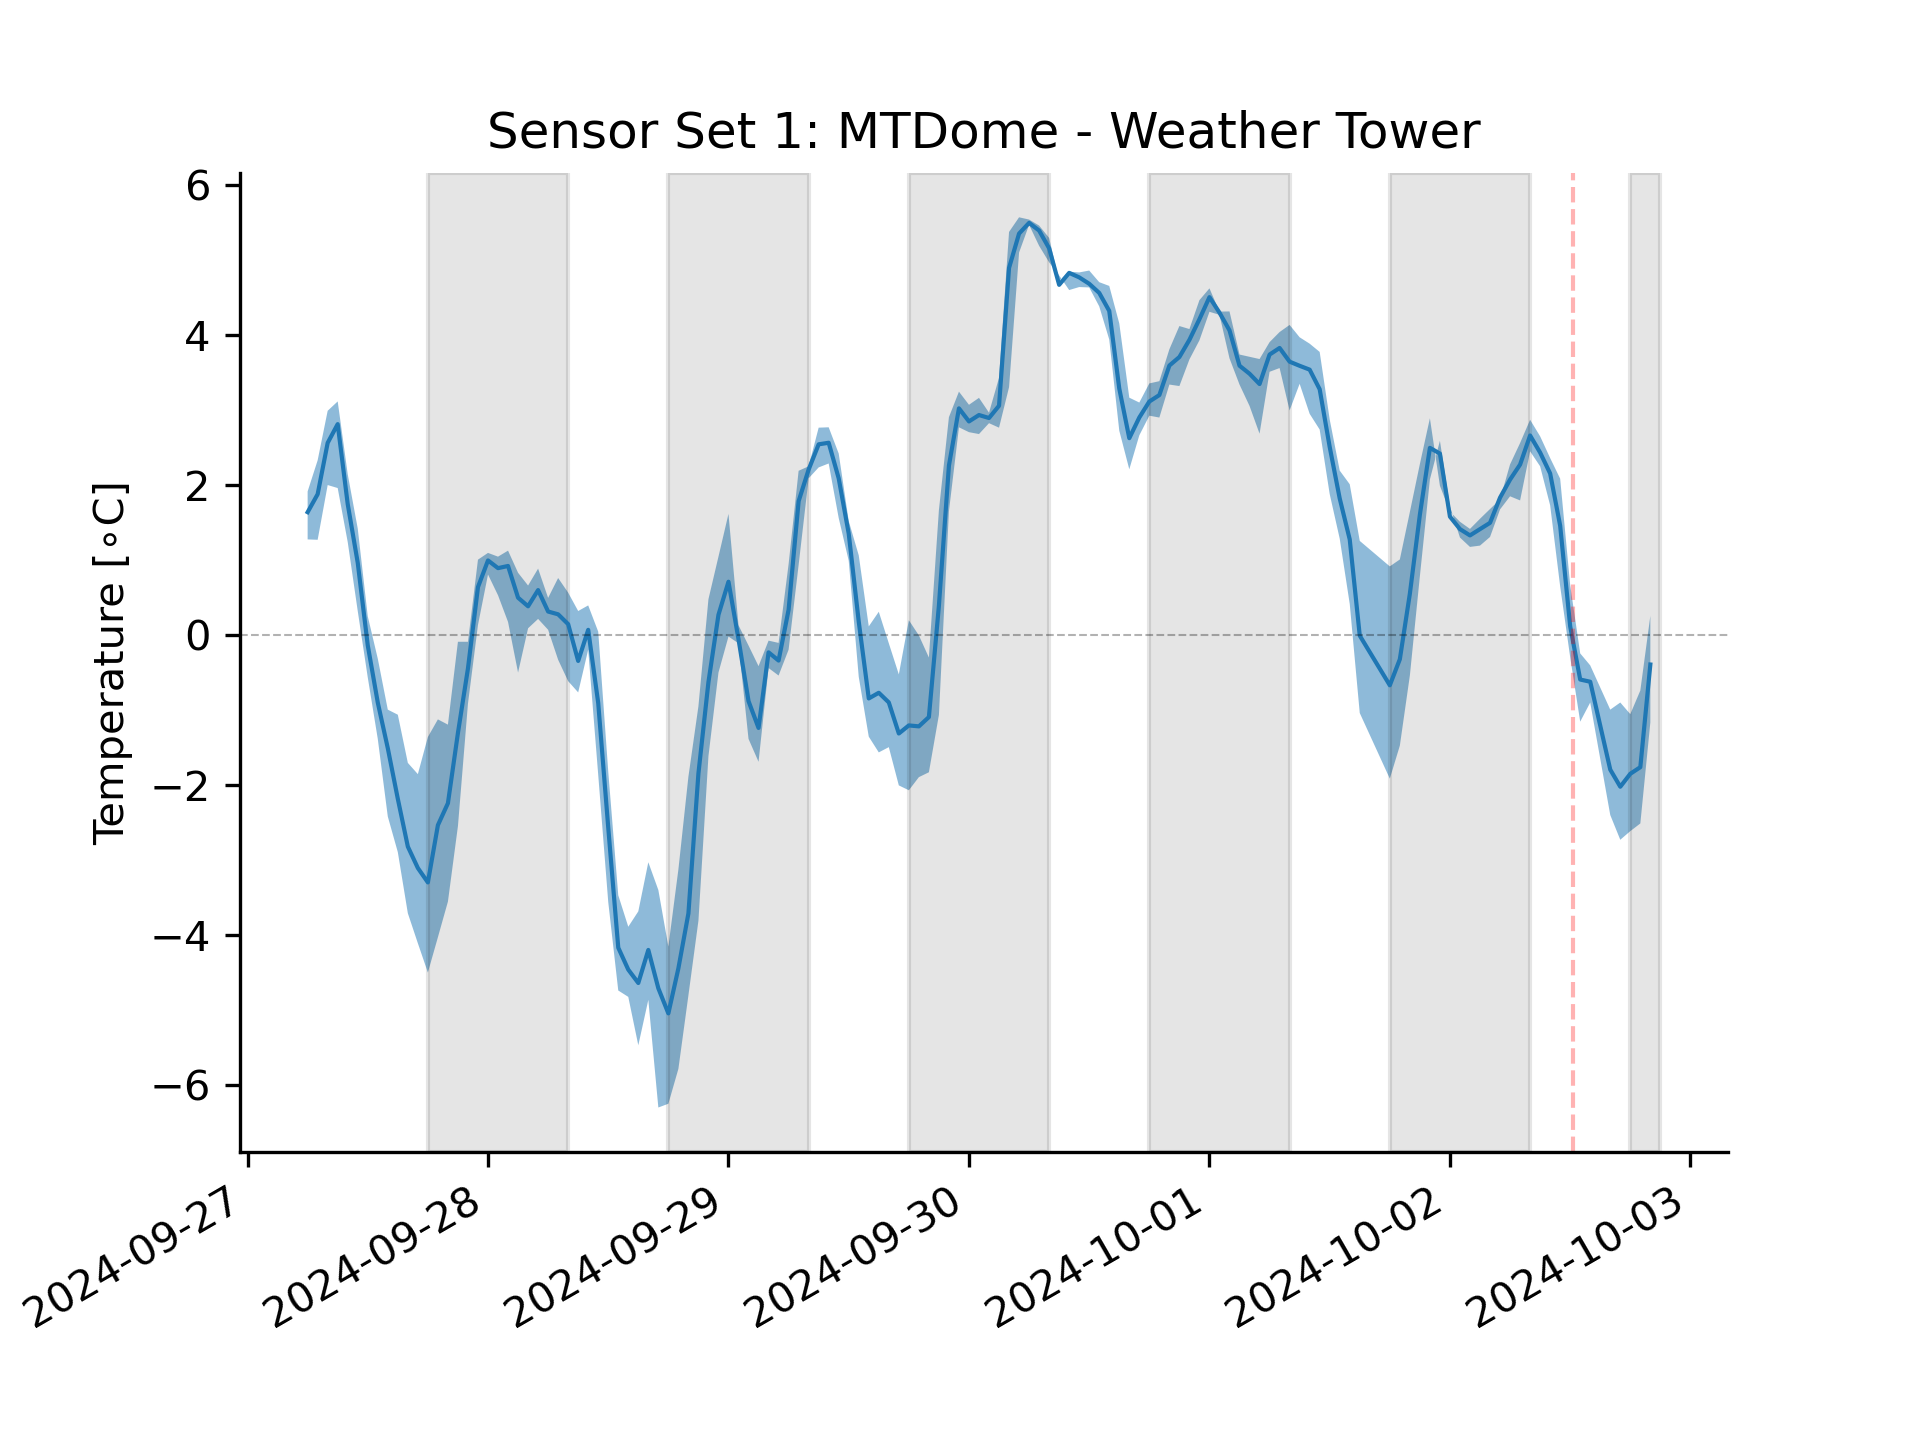
\includegraphics[width=8cm]{SITCOMTN-141_figures/Sensor1_1h_delta_temp_moment.png}
  \caption{Temperature difference between dome and weather station, dashed red lines indicate the first mirror stress thermal requirement, temperature minimum and maximun values are shown. \textit{Left:} Period studied from August 14 to October 2 2024. \textit{Right:} The week prior mirror transportation is shown, day/night time indicated as shaded areas. The vertical dashed line marks the movement start.}
  \label{fig_set1_difference}
\end{figure}

Figure \ref{fig_set1_derivative} shows the derivative per hour on the mirror ambient temperature \footnote{The analysis shown here used \texttt{python.pandas.diff} package (backward finite difference) to calculate the derivatives. To ensuring computational reproducibility the \texttt{python.numpy.gradient} package was also used. The results were comparable.}. The second thermal stress requirement (temperature in the mirror can not change more than 1\,\textdegree C per hour) was surprased a couple of times in the period studied. A closer look of both events (August 20 and September 25) is shown on Figure \ref{fig_set1_derivative_events}. As previously mentioned, the fast and notorious change in temperature inside the dome was related with flushing through air circulation (aperture shutter/RAD door/p-flow rail).

\begin{figure}[h!]
  \centering
  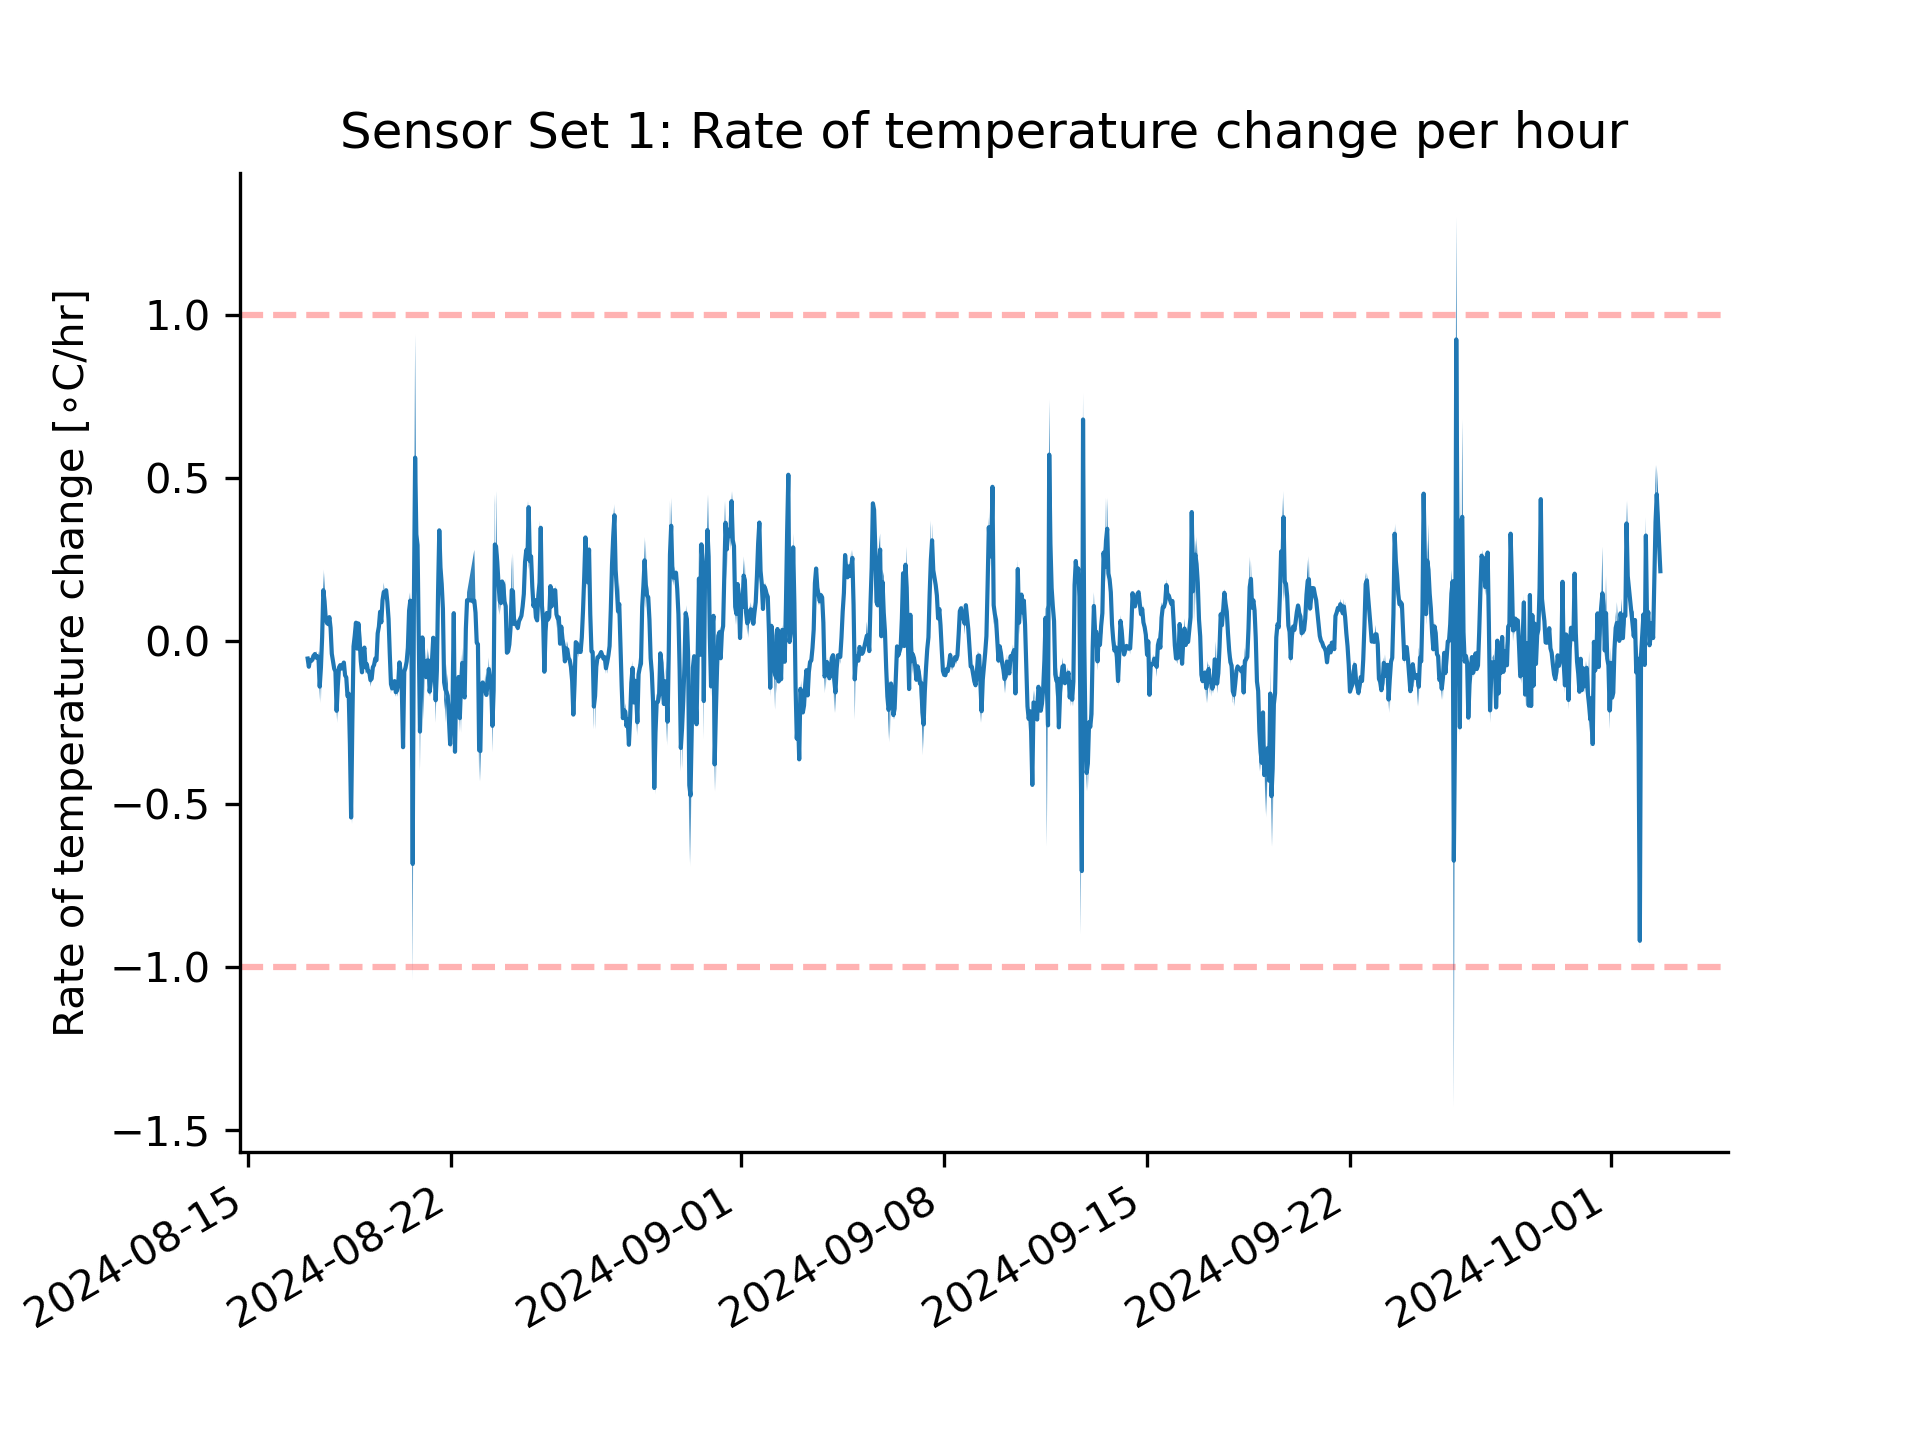
\includegraphics[width=12cm]{SITCOMTN-141_figures/Sensor1_1h_temp_derivative.png}
  \caption{Rate of temperature change per hour on the M1M3 sensor inside the dome, dashed red lines indicate the second mirror stress thermal requirement, temperature minimum and maximun values are shown. Period studied from August 14 to October 2 2024. }
  \label{fig_set1_derivative}
\end{figure}

\begin{figure}[h!]
  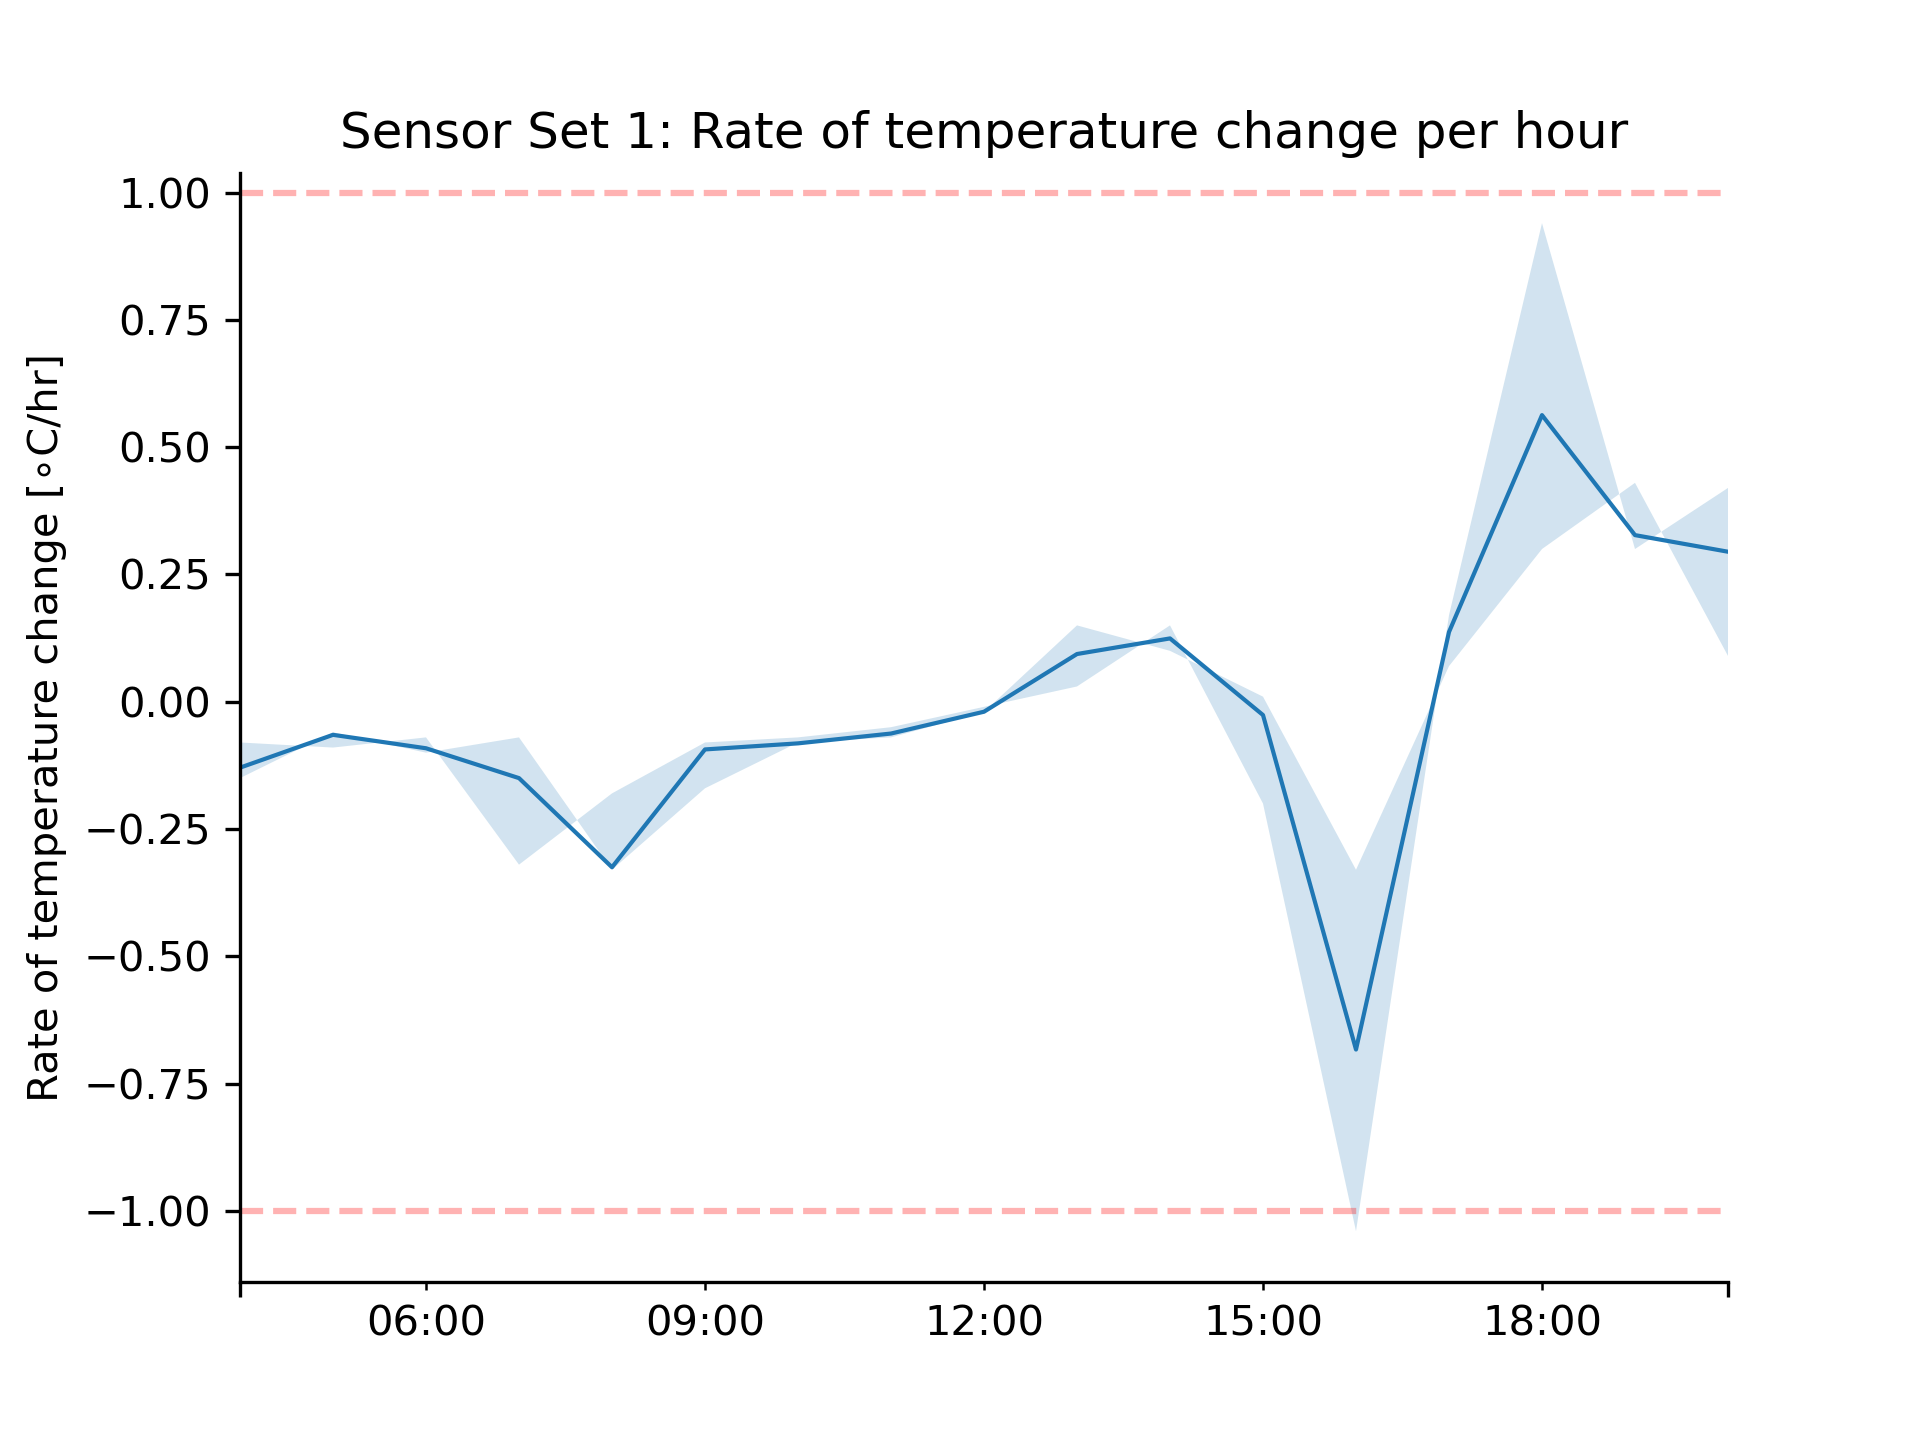
\includegraphics[width=8cm]{SITCOMTN-141_figures/Sensor1_1h_temp_derivative_e1.png}
  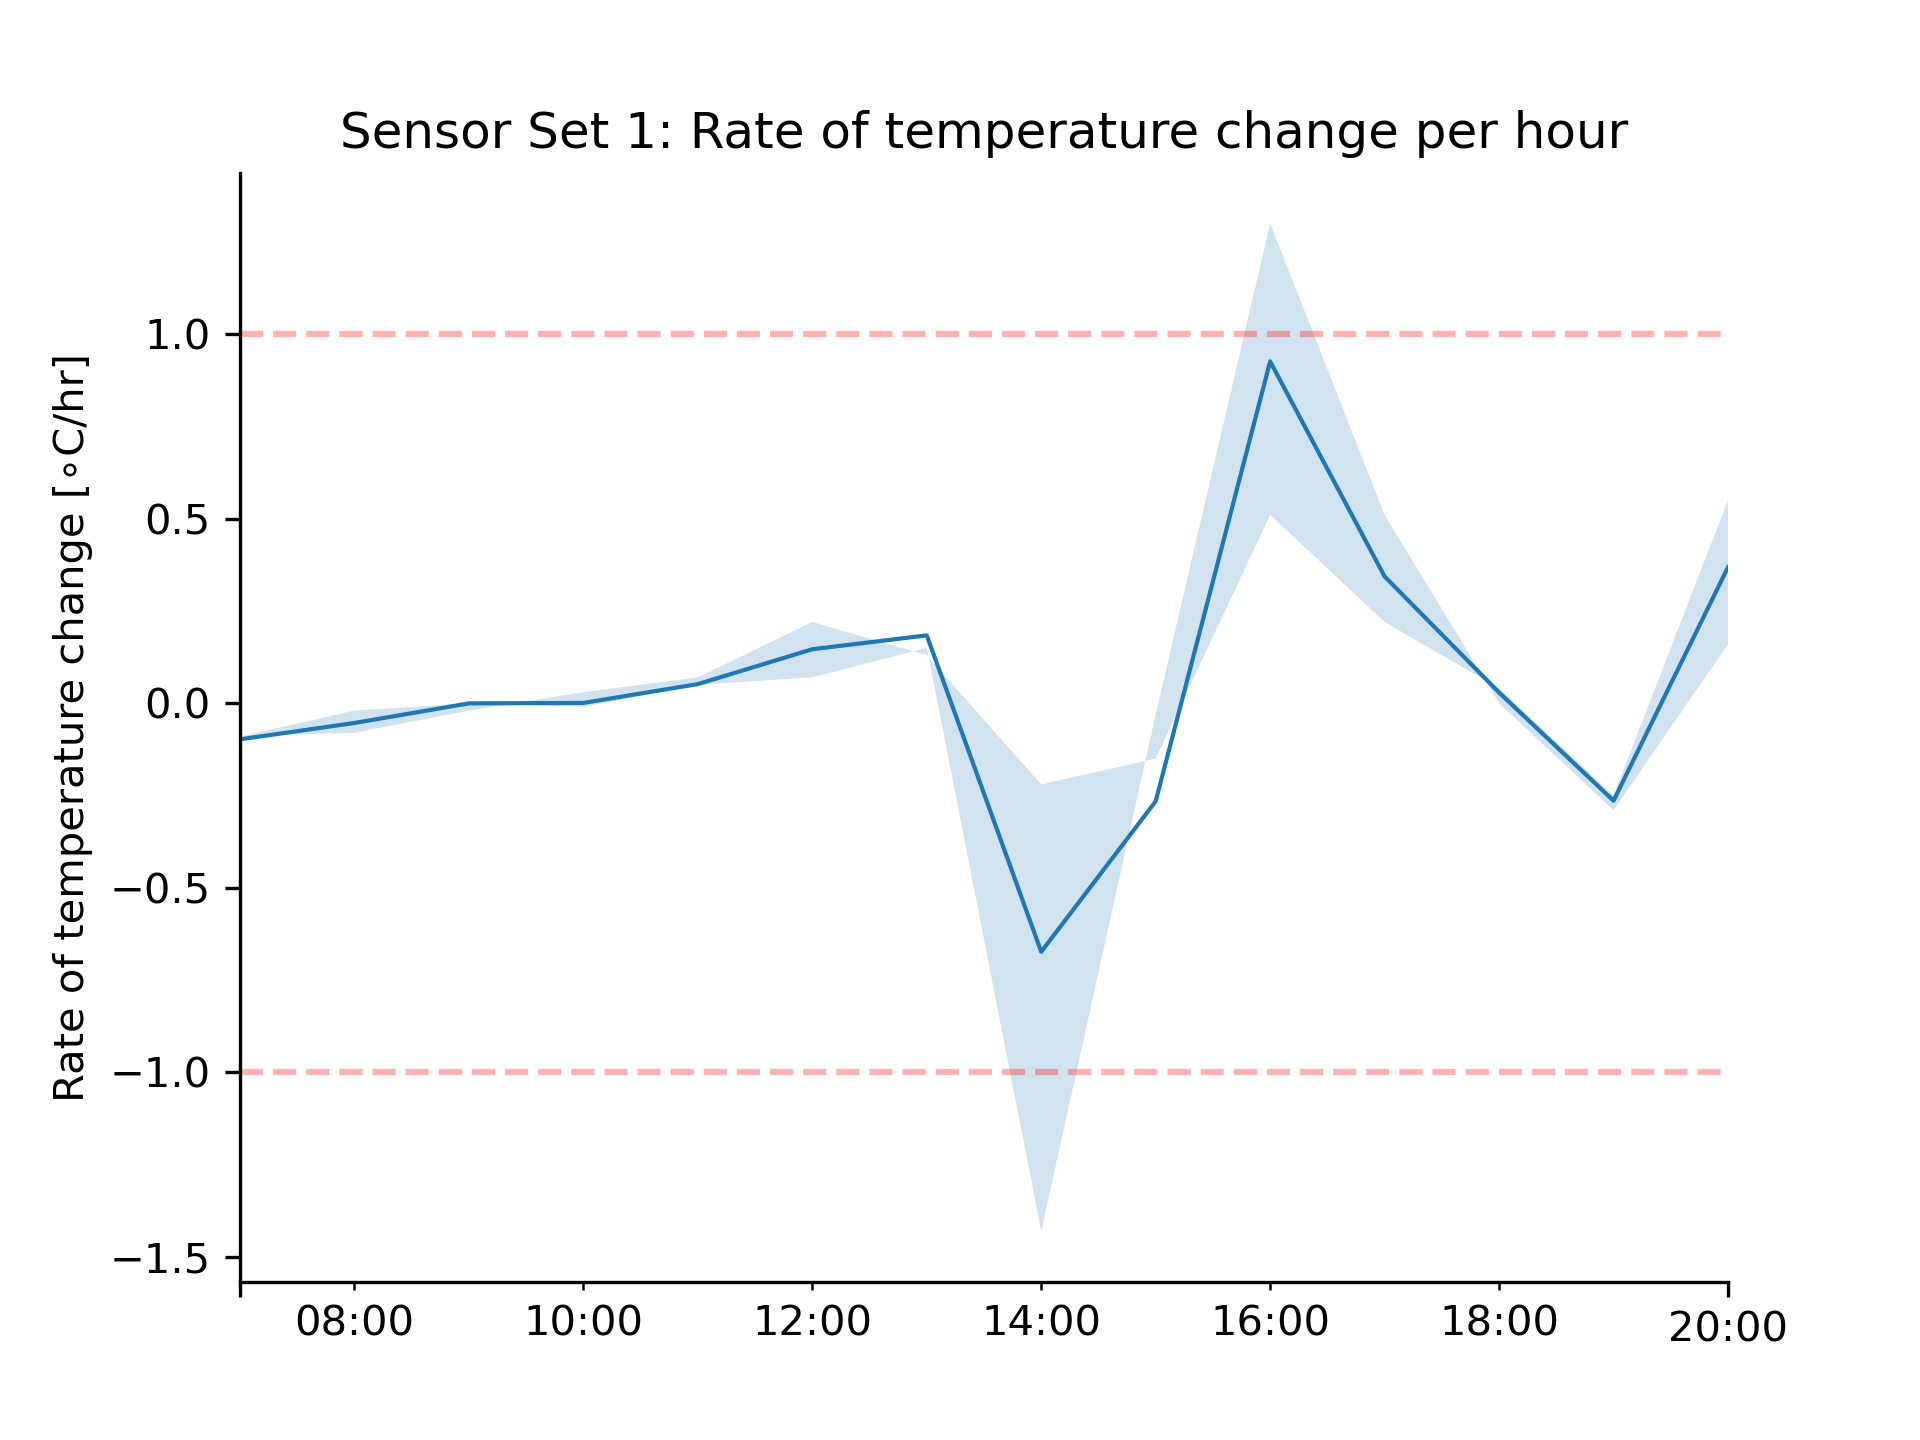
\includegraphics[width=8cm]{SITCOMTN-141_figures/Sensor1_1h_temp_derivative_e2.png}
  \caption{Rate of temperature change per hour on the M1M3 sensor inside the dome, dashed red lines indicate the second mirror stress thermal requirement, temperature minimum and maximun values are shown. \textit{Left:} Detail on the August 20 2024 event. \textit{Right:} Detail on the September 25 2024 event.}
  \label{fig_set1_derivative_events}
\end{figure}

A dedicated \href{https://summit-lsp.lsst.codes/chronograf/sources/1/dashboards/349?refresh=Paused&lower=2024-09-21T03%3A00%3A00.000Z&upper=2024-09-23T03%3A00%3A00.000Z}{Chronograf dashboard} including the relevant figures was created for the day of transportation.

\subsection{Sensor Set 2: Local temperature loggers.}
The sensors were studied from September 26 until October 2 when the mirror was moved from L3 to the dome. Figure \ref{fig_set2_raw} shows the temperature data from the local loggers. Three of them were monitoring different cell mirror locations: the center and the extremes on its $x$-axis. Three additional loggers were focused in monitoring the M1M3 ambient temperature. They were located on the cell exterior, one of the L3 walls and the p-flow (lift). We can see that the internal cell temperatures follow in general the same trend with the exception of three events identified as thermal flushing events inside L3. There is no an apparent gradient in temperature on the mirror axial extremes. Regarding the environmental logger temperatures (M1M3 exterior, L3 ambient and p-flow) the dispersion among them is larger. The difference between the M1M3 cell exterior logger and the ones at the cell interior was $\lesssim$2\,\textdegree C in the period studied. It is worth to note how the p-flow temperature thermalizes with the L3 ambient when the p-flow roll up doors are manipulated.

\begin{figure}[h!]
  \centering
  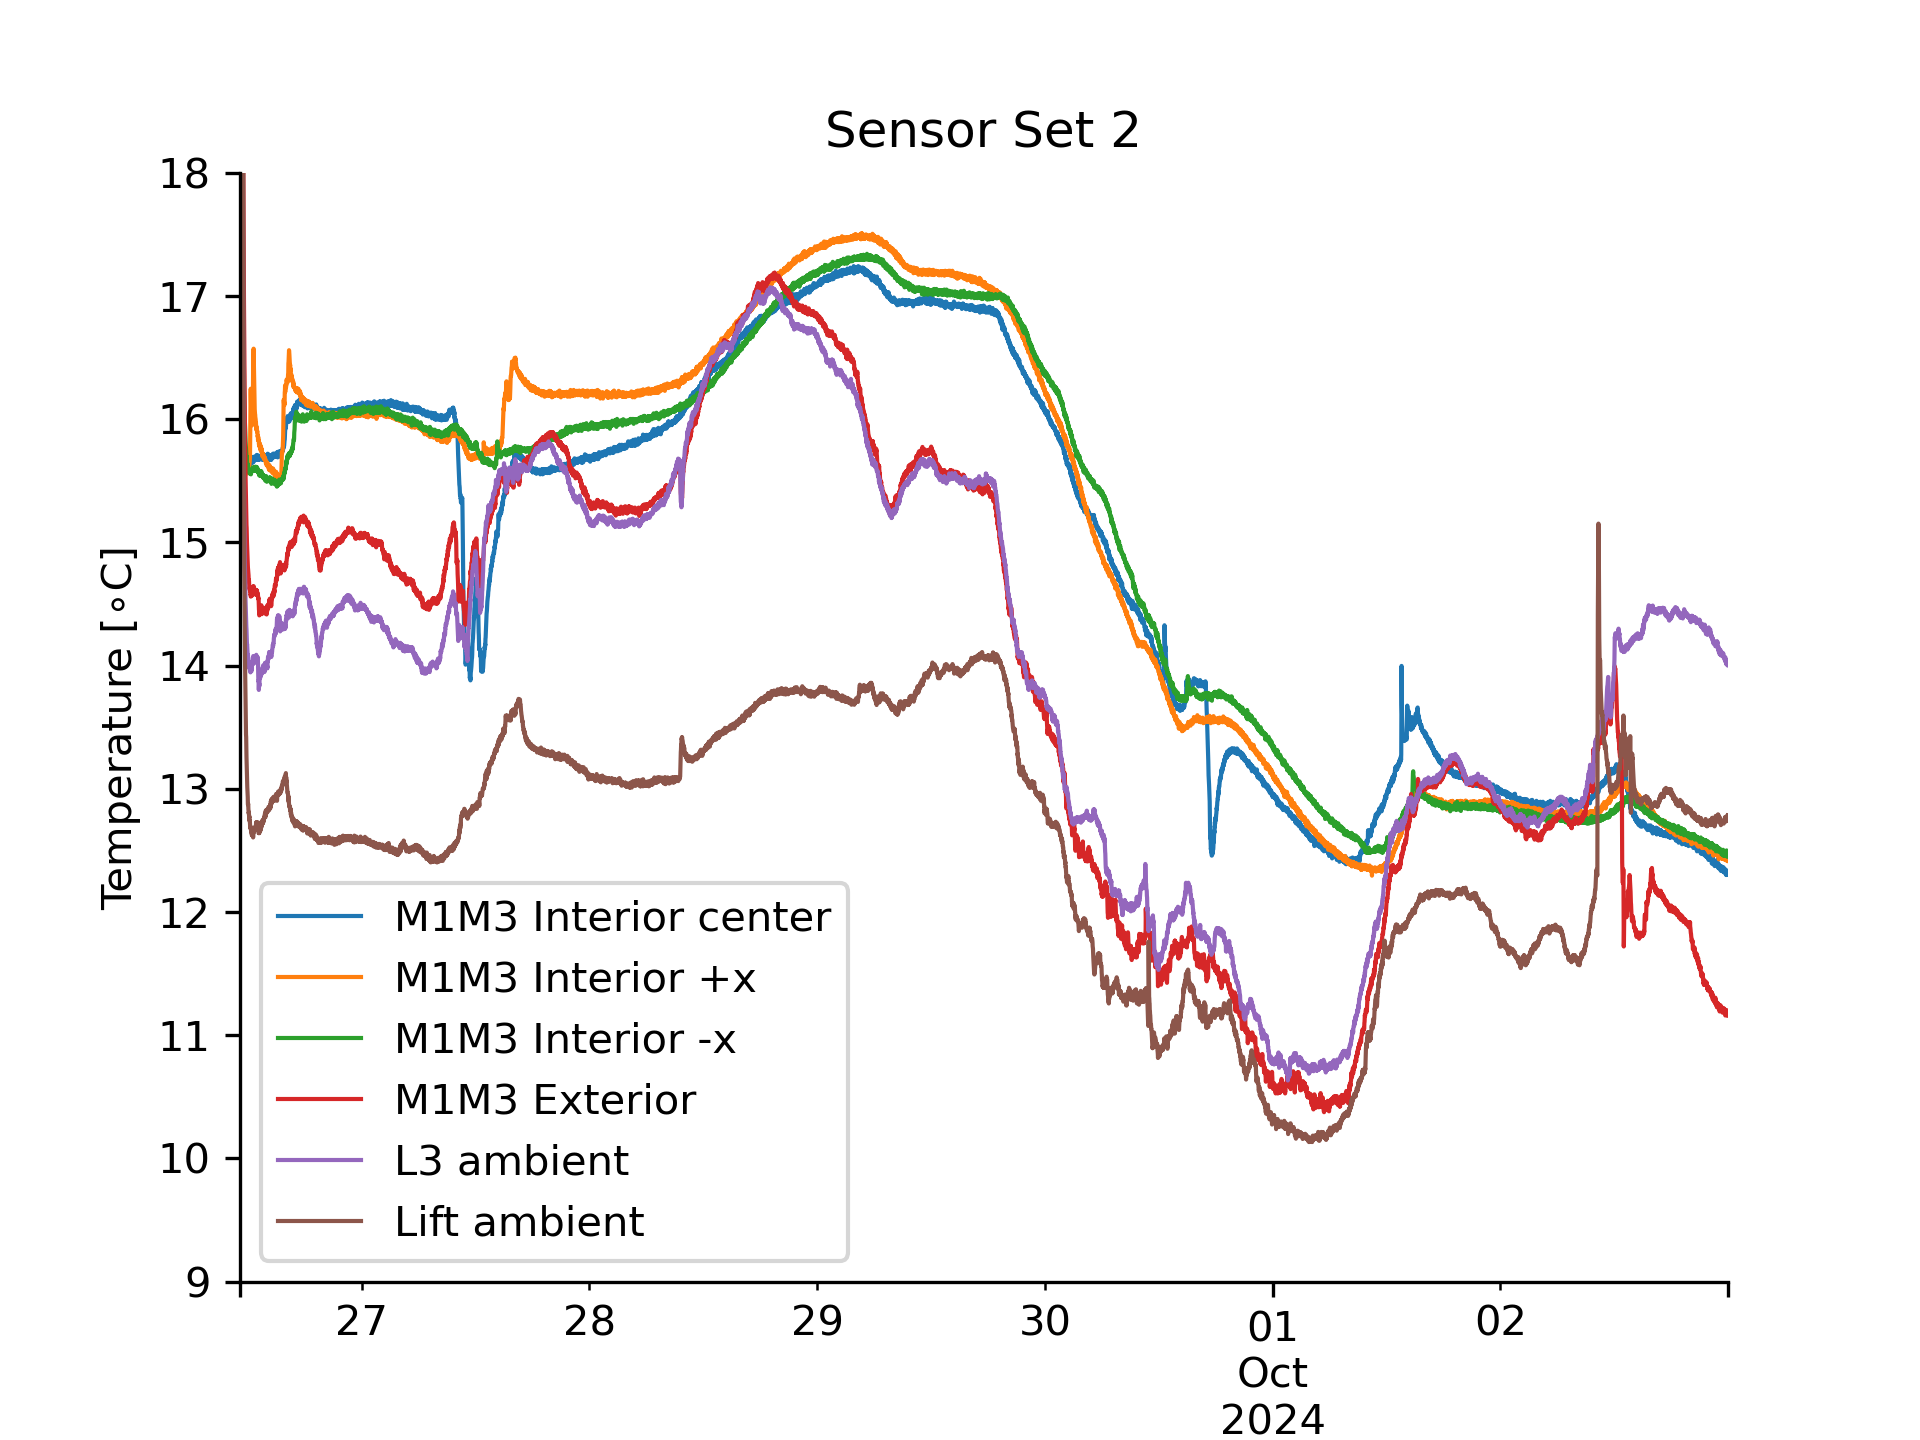
\includegraphics[width=11cm]{SITCOMTN-141_figures/Sensor2_raw.png}
  \caption{Temperature loggers on different mirror locations, temperature minimum and maximun values are shown. Period studied from September 26 to October 2 2024. }
  \label{fig_set2_raw}
\end{figure}

\begin{figure}[h!]
  \centering 
  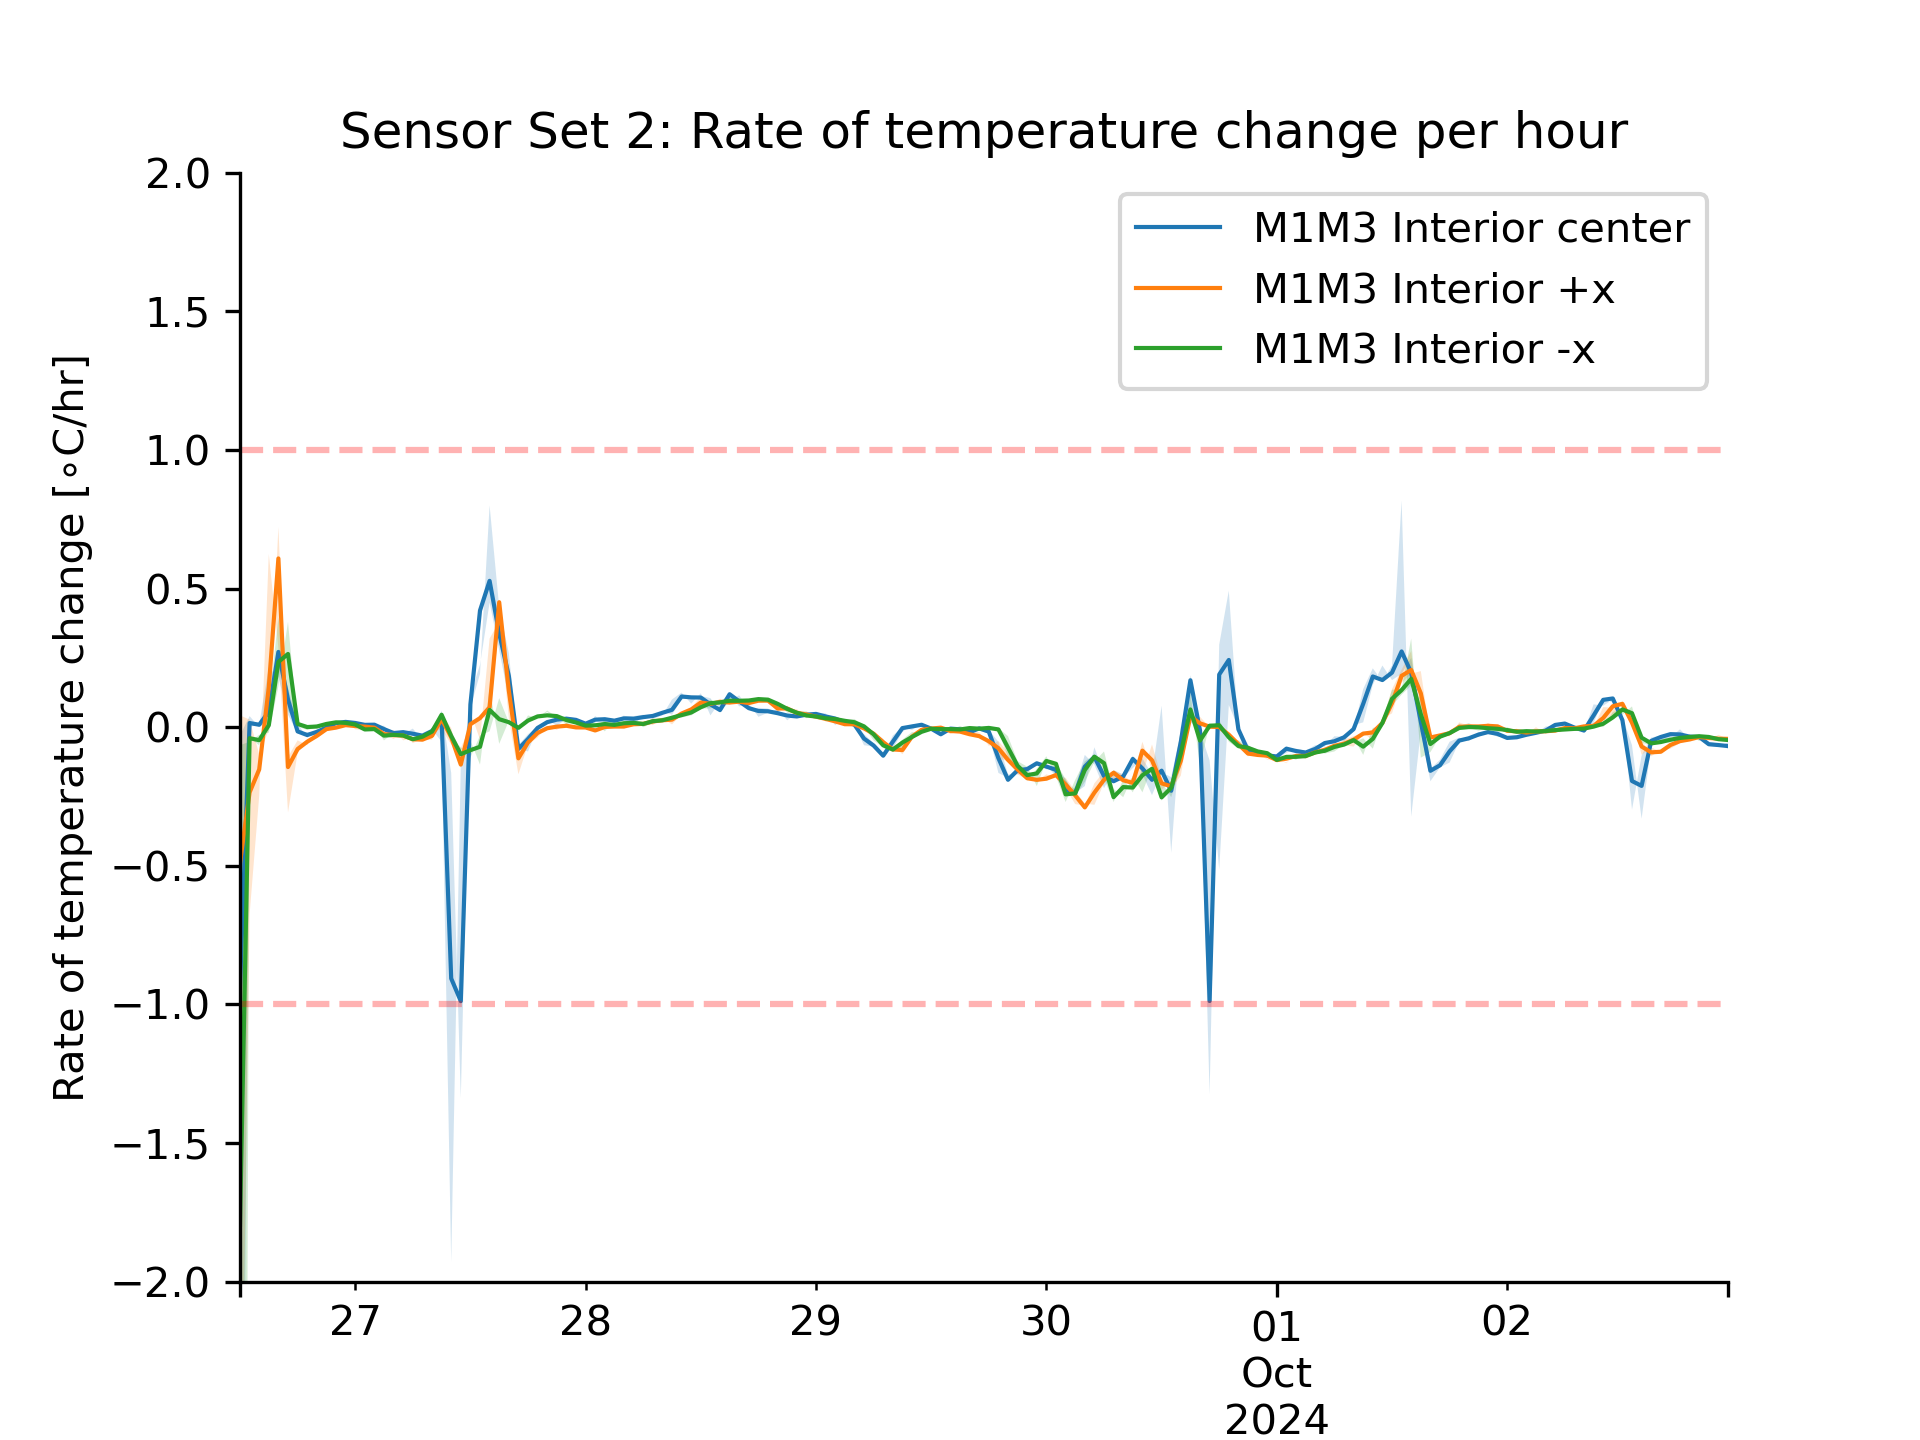
\includegraphics[width=11cm]{SITCOMTN-141_figures/Sensor2_1h_temp_derivative_int_center.png}
  \caption{Rate of temperature change per hour on the M1M3 internal cell loggers, dashed red lines indicate the second mirror stress thermal requirement, temperature minimum and maximun values are shown.}
  \label{fig_set2_derivative}
\end{figure}

In terms of the second thermal stress requirement for M1M3 (rate of temperature change per hour), the temperature gradient on the local temperature loggers can be seen on Figure \ref{fig_set2_derivative}. The loggers that are monitoring the M1M3 cell center and its axial extremes surprassed the limits ($\pm$1\,\textdegree C) in a couple of ocassions. Both episodies were traced back and were related with the aperture of the rear access door (RAD) at the Simonyi telescope dome.

\newpage
\section{Conclusions}
In the previous weeks to the M1M3 movement, we had gradient excursions up to 1\,\textdegree C and temperature differences (inside/outside dome) surpasing the $\pm$5\,\textdegree C limit. Those events were generally linked with dome/L3 thermal flushing using either the main shutters, the RAD or the roll up door at L3. On the date and time of the mirror transportation, the thermal strees requirements for M1M3 were fulfilled. Since the mirror now remains parked on the Telescope Mount Assembly (TMA) inside the dome, the largest impact on M1M3 temperature changes are dome aperture mechanisms unless the M1M3 thermal system is on place. 


\section{}

\appendix
% Include all the relevant bib files.
% https://lsst-texmf.lsst.io/lsstdoc.html#bibliographies
%\section{References} \label{sec:bib}
%\renewcommand{\refname}{} % Suppress default Bibliography section
%\bibliography{local,lsst,lsst-dm,refs_ads,refs,books}

% Make sure lsst-texmf/bin/generateAcronyms.py is in your path
\section{Acronyms} \label{sec:acronyms}
\addtocounter{table}{-1}
\begin{longtable}{p{0.145\textwidth}p{0.8\textwidth}}\hline
\textbf{Acronym} & \textbf{Description}  \\\hline

ESS & Environmental Sensors Support \\\hline
L3 & Lens 3 \\\hline
M1M3 & Primary Mirror Tertiary Mirror \\\hline
OBS & Organisation Breakdown Structure \\\hline
RAD & Rear Access Door \\\hline
SE & System Engineering \\\hline
SITCOM & System Integration, Test and Commissioning \\\hline
TMA & Telescope Mount Assembly \\\hline
UMA & Air Improvement Unit (Spanish) \\\hline
UPS & uninterruptible power supply \\\hline
\end{longtable}

% If you want glossary uncomment below -- comment out the two lines above
%\printglossaries

\end{document}
